\chapter{Work, Power, and the Work-Energy Theorem}
\label{ch:work_energy}
\begin{chapterintro}
\textbf{You will learn to:} define work as a line integral; calculate instantaneous and average power; apply the Work-Energy Theorem for particles; determine the work done by gravity, springs, and friction; and solve classic problems including vertical loops, detachment from surfaces, and resistive forces.
\end{chapterintro}

\section{Definition of Work}

When a force $\vec{F}$ acts on a material point undergoing an infinitesimal displacement $\dd\vec{r}$, the \textbf{elementary mechanical work} done by $\vec{F}$ is the scalar product:
\[
\boxed{\dd W = \vec{F}\cdot\dd\vec{r} = F_x\,\dd x + F_y\,\dd y + F_z\,\dd z = F\,\dd s\cos\theta,}
\]
where $\theta$ is the angle between $\vec{F}$ and the displacement tangent $\dd\vec{r}$, and $\dd s = \norm{\dd\vec{r}}$ is the arc length.

For a finite displacement along a curve $\mathcal{C}$ from initial point $A$ to final point $B$, the total work is the \textbf{line integral}:
\[
\boxed{W_{A\to B}(\vec{F}) = \int_{\mathcal{C}} \vec{F}\cdot\dd\vec{r}.}
\]
Work is measured in \textbf{joules} ($1\ \mathrm{J} = 1\ \mathrm{N\,m} = 1\ \mathrm{kg\,m^2\,s^{-2}}$).

\begin{figure}[htbp]
\centering
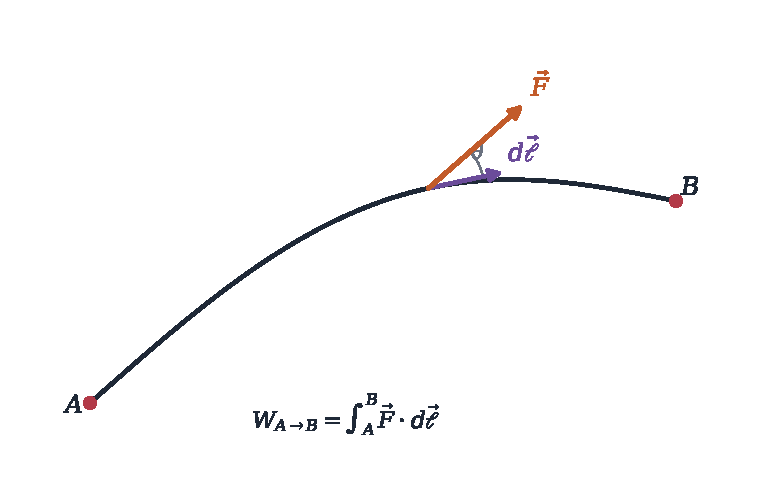
\includegraphics[width=0.74\textwidth]{figures/18_work_path.pdf}
\caption{The line integral of force $\vec{F}$ along a curved trajectory from point $A$ to point $B$. The tangential projection $F_t = \vec{F}\cdot\vec{u}_t$ contributes to the work.}
\label{fig:work_path}
\end{figure}

\begin{keyidea}[Sign of Mechanical Work]
\begin{itemize}[leftmargin=1.4em,itemsep=2pt]
  \item \textbf{Motive work} ($W > 0$): $\theta < 90^\circ$ ($\vec{F}\cdot\vec{v} > 0$). The force accelerates the particle, adding energy.
  \item \textbf{Resistive work} ($W < 0$): $\theta > 90^\circ$ ($\vec{F}\cdot\vec{v} < 0$). The force opposes motion, removing energy (e.g. friction).
  \item \textbf{Zero work} ($W = 0$): $\theta = 90^\circ$ ($\vec{F}\perp\vec{v}$). Forces perpendicular to velocity do \textbf{no work}!
  Examples: normal reactions from smooth rigid surfaces, magnetic forces ($\vec{F} = q\vec{v}\times\vec{B}$), and the Coriolis force ($\vec{F}_{ic} = -2m\vec{\Omega}\times\vec{v}_r$).
\end{itemize}
\end{keyidea}

\section{Instantaneous Power}

The rate at which work is performed with respect to time is the \textbf{instantaneous power}:
\[
\boxed{P(t) = \frac{\dd W}{\dd t} = \vec{F}\cdot\frac{\dd\vec{r}}{\dd t} = \vec{F}\cdot\vec{v}.}
\]
Power is measured in \textbf{watts} ($1\ \mathrm{W} = 1\ \mathrm{J\,s^{-1}} = 1\ \mathrm{kg\,m^2\,s^{-3}}$).

\section{The Work-Energy Theorem}

The \textbf{kinetic energy} of a material point of mass $m$ moving at speed $v$ is:
\[
\boxed{E_c = \frac{1}{2}m v^2 = \frac{p^2}{2m}.}
\]
Taking the time derivative of $E_c$:
\[
\frac{\dd E_c}{\dd t} = \frac{\dd}{\dd t}\left(\frac{1}{2}m\vec{v}\cdot\vec{v}\right) = m\vec{v}\cdot\frac{\dd\vec{v}}{\dd t} = \vec{v}\cdot(m\vec{a}) = \vec{v}\cdot\sum\vec{F} = P_{\text{net}}(t).
\]
Multiplying by $\dd t$:
\[
\dd E_c = \dd W_{\text{net}} = \sum\vec{F}\cdot\dd\vec{r}.
\]
Integrating between points $A$ and $B$ gives the \textbf{Work-Energy Theorem} (\emph{Théorème de l'énergie cinétique}):
\[
\boxed{\Delta E_c = E_c(B) - E_c(A) = \frac{1}{2}m v_B^2 - \frac{1}{2}m v_A^2 = W_{A\to B}\left(\sum\vec{F}\right).}
\]
\begin{keyidea}[Power of the Work-Energy Theorem]
The work-energy theorem allows us to find speeds directly from displacements \textbf{without needing to integrate Newton's second law with respect to time}!
\end{keyidea}

\section{Work Done by Common Forces}

\begin{center}
\renewcommand{\arraystretch}{1.3}
\begin{tabular}{@{}lll@{}}
\toprule
\textbf{Force} & \textbf{Expression} & \textbf{Work $W_{A\to B}$} \\
\midrule
Uniform gravity & $\vec{P} = -mg\khat$ & $-mg(z_B - z_A)$ \\
Ideal spring & $\vec{F}_s = -k x\ihat$ & $-\frac{1}{2}k(x_B^2 - x_A^2)$ \\
Kinetic friction & $\vec{f}_k = -\mu_k N\,\vec{u}_t$ & $-\int_A^B \mu_k N\,\dd s = -\mu_k N\,d$ (along straight line) \\
Normal reaction & $\vec{N}\perp\vec{v}$ & $0$ \\
\bottomrule
\end{tabular}
\end{center}

\section{Worked Examples}

\begin{worked}[Braking distance with kinetic friction]
A car travels at $v_0 = 90.0\ \mathrm{km\,h^{-1}} = 25.0\ \mathrm{m\,s^{-1}}$ on a horizontal road. The driver slams on the brakes, locking all four wheels. The coefficient of kinetic friction between tires and asphalt is $\mu_k = 0.700$. Using the work-energy theorem, find the stopping distance $d$.
\end{worked}

\begin{solution}{12.1}
The forces acting on the car during braking are:
\begin{itemize}[leftmargin=1.4em,itemsep=2pt]
  \item Vertical: gravity $\vec{P} = -mg\jhat$ and normal force $\vec{N} = N\jhat$. Since $a_y = 0$, $N = mg$.
  \item Horizontal: kinetic friction $\vec{f}_k = -\mu_k N\ihat = -\mu_k mg\ihat$.
\end{itemize}
Work done:
\begin{itemize}[leftmargin=1.4em,itemsep=2pt]
  \item $W(\vec{P}) = 0$ and $W(\vec{N}) = 0$ (perpendicular to displacement).
  \item $W(\vec{f}_k) = -f_k d = -\mu_k mg d$.
\end{itemize}
By the work-energy theorem between the initial state ($v_A = v_0$) and final stopped state ($v_B = 0$):
\[
\Delta E_c = 0 - \frac{1}{2}m v_0^2 = W_{\text{net}} = -\mu_k mg d.
\]
The mass $m$ cancels:
\[
\frac{1}{2}v_0^2 = \mu_k g d \implies \boxed{d = \frac{v_0^2}{2\mu_k g}.}
\]
Computing:
\[
d = \frac{(25.0)^2}{2(0.700)(9.81)} = \frac{625}{13.734} \approx \mathbf{45.5\ \mathrm{m}.}
\]
\end{solution}

\begin{worked}[The vertical loop-the-loop]
A small roller coaster car of mass $m$ starts from rest at height $h$ and slides down a frictionless track ending in a vertical circular loop of radius $R$.
(a) Find the speed of the car at the highest point of the loop (point $T$, at height $2R$).
(b) Find the normal force $N_T$ exerted by the track at the top.
(c) Deduce the minimum release height $h_{\min}$ to complete the loop without leaving the track.
\end{worked}

\begin{solution}{12.2}
(a) Applying the work-energy theorem between the release point $A$ (height $h$, $v_A = 0$) and the top of the loop $T$ (height $2R$, speed $v_T$):
Since the normal force $\vec{N}\perp\vec{v}$ does no work ($W(\vec{N}) = 0$), only gravity performs work:
\[
W_{A\to T}(\vec{P}) = -mg(z_T - z_A) = -mg(2R - h) = mg(h - 2R).
\]
Thus:
\[
\Delta E_c = \frac{1}{2}m v_T^2 - 0 = mg(h - 2R) \implies \boxed{v_T^2 = 2g(h - 2R).}
\]

(b) At point $T$, both gravity and the track normal force $\vec{N}_T$ point vertically downward toward the center of the circle:
\[
\sum F_{\text{rad}} = N_T + mg = m\frac{v_T^2}{R}.
\]
Solving for $N_T$:
\[
N_T = m\frac{v_T^2}{R} - mg = \frac{m}{R}\left[ 2g(h - 2R) \right] - mg = mg\left( \frac{2h}{R} - 5 \right).
\]

(c) The car remains on the track as long as the normal force is non-negative ($N_T \ge 0$):
\[
mg\left( \frac{2h}{R} - 5 \right) \ge 0 \implies \frac{2h}{R} \ge 5 \implies \boxed{h_{\min} = \frac{5}{2}R = 2.5R.}
\]
At this minimum height, the speed at the top is $v_T = \sqrt{gR}$, and the car is momentarily in free fall ($N_T = 0$).
\end{solution}

\section{Exercises and Step-by-Step Solutions}

\begin{exercise}{\warm\ Pulling a crate at an angle}
A worker pulls a crate of mass $m=40.0\ \mathrm{kg}$ across a smooth horizontal floor over a distance $d=15.0\ \mathrm{m}$ by applying a force of magnitude $F=120\ \mathrm{N}$ via a rope angled at $\alpha=30.0^\circ$ above the horizontal.
(a) Compute the work done by each force: the pulling force $\vec{F}$, gravity $\vec{P}$, and normal force $\vec{N}$.
(b) If the crate starts from rest, find its final speed $v_f$ using the work-energy theorem.
\end{exercise}

\begin{tabletworkspace}[5.0cm]
\end{tabletworkspace}

\begin{solution}{12.1}
(a) Work calculations:
\begin{itemize}[leftmargin=1.4em,itemsep=2pt]
  \item Pulling force: $W(\vec{F}) = F d\cos\alpha = (120)(15.0)\cos 30.0^\circ = 1800\times 0.8660 \approx \mathbf{1559\ \mathrm{J}} = 1.56\ \mathrm{kJ}$.
  \item Gravity: $\vec{P} = -mg\jhat$ is perpendicular to displacement $\dd\vec{r} = \dd x\ihat \implies W(\vec{P}) = \mathbf{0\ \mathrm{J}}$.
  \item Normal force: $\vec{N} = N\jhat \perp \dd\vec{r} \implies W(\vec{N}) = \mathbf{0\ \mathrm{J}}$.
\end{itemize}

(b) Total net work: $W_{\text{net}} = 1559\ \mathrm{J}$.
By the work-energy theorem:
\[
\Delta E_c = \frac{1}{2}m v_f^2 - 0 = W_{\text{net}} \implies v_f = \sqrt{\frac{2 W_{\text{net}}}{m}} = \sqrt{\frac{2\times 1559}{40.0}} = \sqrt{77.94} \approx \mathbf{8.83\ \mathrm{m\,s^{-1}}.}
\]
\end{solution}

\begin{exercise}{\warm\ Cruising power of an automobile}
A car of mass $m=1400\ \mathrm{kg}$ cruises at a constant speed of $v=108\ \mathrm{km\,h^{-1}} = 30.0\ \mathrm{m\,s^{-1}}$ on a flat horizontal highway. The total resistance force opposing its motion (aerodynamic drag plus rolling resistance) is $F_{\text{res}} = 650\ \mathrm{N}$.
(a) What driving force $F_{\text{engine}}$ must the engine deliver at constant speed?
(b) Calculate the mechanical power output $P$ delivered to the wheels in kilowatts and horsepower ($1\ \mathrm{hp} = 746\ \mathrm{W}$).
(c) If the car now climbs an uphill slope of grade $5.0\%$ ($\sin\alpha \approx 0.050$), what power is needed to maintain the same speed?
\end{exercise}

\begin{tabletworkspace}[5.5cm]
\end{tabletworkspace}

\begin{solution}{12.2}
(a) At constant speed, $\vec{a} = \vzero$, so $\sum\vec{F} = \vzero$:
\[
F_{\text{engine}} - F_{\text{res}} = 0 \implies F_{\text{engine}} = F_{\text{res}} = \mathbf{650\ \mathrm{N}.}
\]

(b) Mechanical power:
\[
P = F_{\text{engine}} v = (650\ \mathrm{N})(30.0\ \mathrm{m\,s^{-1}}) = 19500\ \mathrm{W} = \mathbf{19.5\ \mathrm{kW}.}
\]
In horsepower:
\[
P_{\text{hp}} = \frac{19500}{746} \approx \mathbf{26.1\ \mathrm{hp}.}
\]

(c) On the $5\%$ incline, gravity adds a component opposing motion: $P_\parallel = mg\sin\alpha$.
\[
P_\parallel = (1400)(9.81)(0.050) = 686.7\ \mathrm{N}.
\]
The new required engine thrust is:
\[
F_{\text{new}} = F_{\text{res}} + mg\sin\alpha = 650 + 686.7 = 1336.7\ \mathrm{N}.
\]
The required power is:
\[
P_{\text{climb}} = F_{\text{new}} v = (1336.7)(30.0) = 40101\ \mathrm{W} \approx \mathbf{40.1\ \mathrm{kW}} \approx \mathbf{53.8\ \mathrm{hp}.}
\]
The required power more than doubles to climb the incline!
\end{solution}

\begin{exercise}{\core\ Mass sliding down a rough ramp}
A block of mass $m=3.00\ \mathrm{kg}$ is released from rest at the top of a ramp inclined at $\theta=37.0^\circ$ of length $L=5.00\ \mathrm{m}$. The coefficient of kinetic friction is $\mu_k=0.250$.
(a) Calculate the work done by gravity $W_g$ as the block slides down the entire ramp.
(b) Calculate the work done by friction $W_f$.
(c) Using the work-energy theorem, find the speed of the block at the bottom of the ramp.
\end{exercise}

\begin{tabletworkspace}[5.5cm]
\end{tabletworkspace}

\begin{solution}{12.3}
(a) The vertical height difference is $h = L\sin\theta = 5.00\sin 37.0^\circ = 5.00(0.6018) = 3.009\ \mathrm{m}$.
Work done by gravity:
\[
W_g = +mgh = (3.00)(9.81)(3.009) \approx \mathbf{88.56\ \mathrm{J}.}
\]

(b) The normal force perpendicular to the ramp is $N = mg\cos\theta$.
The kinetic friction force is $f_k = \mu_k N = \mu_k mg\cos\theta$.
Since friction opposes displacement over length $L$:
\[
W_f = -f_k L = -\mu_k mg\cos\theta\,L = -(0.250)(3.00)(9.81)(\cos 37.0^\circ)(5.00) = -(0.250)(3.00)(9.81)(0.7986)(5.00) \approx \mathbf{-29.38\ \mathrm{J}.}
\]

(c) Net work:
\[
W_{\text{net}} = W_g + W_f = 88.56 - 29.38 = 59.18\ \mathrm{J}.
\]
By the work-energy theorem:
\[
\frac{1}{2}m v_f^2 - 0 = W_{\text{net}} \implies v_f = \sqrt{\frac{2 W_{\text{net}}}{m}} = \sqrt{\frac{2\times 59.18}{3.00}} = \sqrt{39.45} \approx \mathbf{6.28\ \mathrm{m\,s^{-1}}.}
\]
\end{solution}

\begin{exercise}{\core\ Vertical spring: maximum stretch}
A mass $m=1.50\ \mathrm{kg}$ is attached to an unstretched vertical spring of stiffness $k=120\ \mathrm{N\,m^{-1}}$ and released from rest.
(a) State all forces acting on the mass and express their work when the spring stretches by a distance $x$.
(b) Use the work-energy theorem to find the maximum extension $x_{\max}$ of the spring.
(c) Compare $x_{\max}$ with the static equilibrium extension $x_{\text{eq}}$. Explain why $x_{\max} = 2x_{\text{eq}}$.
\end{exercise}

\begin{tabletworkspace}[5.5cm]
\end{tabletworkspace}

\begin{solution}{12.4}
(a) Two forces act during the vertical descent by distance $x$:
\begin{itemize}[leftmargin=1.4em,itemsep=2pt]
  \item Gravity: downward displacement by $x \implies W_g = +mgx$.
  \item Spring restoring force: $F_s = -kx$ opposing extension $\implies W_s = -\int_0^x kx'\dd x' = -\frac{1}{2}kx^2$.
\end{itemize}

(b) At maximum extension $x_{\max}$, the mass momentarily comes to rest ($v = 0$):
\[
\Delta E_c = 0 - 0 = 0.
\]
By the work-energy theorem:
\[
W_{\text{net}} = W_g + W_s = mgx_{\max} - \frac{1}{2}kx_{\max}^2 = 0.
\]
Since $x_{\max} \ne 0$:
\[
mg - \frac{1}{2}kx_{\max} = 0 \implies \boxed{x_{\max} = \frac{2mg}{k}.}
\]
Computing:
\[
x_{\max} = \frac{2(1.50)(9.81)}{120} = \frac{29.43}{120} \approx \mathbf{0.245\ \mathrm{m}} = 24.5\ \mathrm{cm}.
\]

(c) At static equilibrium, the net force is zero:
\[
\sum F = mg - kx_{\text{eq}} = 0 \implies x_{\text{eq}} = \frac{mg}{k} = \frac{24.5}{2} = 12.25\ \mathrm{cm}.
\]
Therefore, $x_{\max} = 2x_{\text{eq}}$.
Because the system has no friction, the mass does not stop at equilibrium; when passing through $x_{\text{eq}}$, it has maximum kinetic energy! It overshoots equilibrium by exactly an equal distance $x_{\text{eq}}$, oscillating symmetrically between $x=0$ and $x=2x_{\text{eq}}$.
\end{solution}

\begin{exercise}{\core\ Path-dependent work: conservative vs non-conservative forces}
Consider the force field $\vec{F}(x, y) = y^2\,\ihat + 2xy\,\jhat$ and a second force field $\vec{G}(x, y) = y\,\ihat + 2x\,\jhat$.
(a) Compute the work done by each force along Path 1: straight line from $(0,0)$ to $(1,1)$ ($y = x$).
(b) Compute the work done by each force along Path 2: from $(0,0)$ along the $x$-axis to $(1,0)$, then vertically to $(1,1)$.
(c) State which force is conservative and compute $\vec{\nabla}\times\vec{F}$ and $\vec{\nabla}\times\vec{G}$.
\end{exercise}

\begin{tabletworkspace}[6.5cm]
\end{tabletworkspace}

\begin{solution}{12.5}
(a) Path 1 ($y = x \implies \dd y = \dd x$ from $x=0$ to $x=1$):
\begin{align*}
W_1(\vec{F}) &= \int_0^1 (x^2\,\dd x + 2x^2\,\dd x) = \int_0^1 3x^2\,\dd x = \left[ x^3 \right]_0^1 = \mathbf{1.0\ \mathrm{J}.} \\
W_1(\vec{G}) &= \int_0^1 (x\,\dd x + 2x\,\dd x) = \int_0^1 3x\,\dd x = \left[ \frac{3}{2}x^2 \right]_0^1 = \mathbf{1.5\ \mathrm{J}.}
\end{align*}

(b) Path 2: Segment A: $(0,0)\to(1,0)$ ($y=0, \dd y=0, x: 0\to 1$); Segment B: $(1,0)\to(1,1)$ ($x=1, \dd x=0, y: 0\to 1$):
For $\vec{F}$:
\begin{align*}
W_{2A}(\vec{F}) &= \int_0^1 0^2\,\dd x = 0, \\
W_{2B}(\vec{F}) &= \int_0^1 2(1)y\,\dd y = \left[ y^2 \right]_0^1 = 1.0\ \mathrm{J}. \\
W_2(\vec{F}) &= 0 + 1.0 = \mathbf{1.0\ \mathrm{J}.}
\end{align*}
For $\vec{G}$:
\begin{align*}
W_{2A}(\vec{G}) &= \int_0^1 0\,\dd x = 0, \\
W_{2B}(\vec{G}) &= \int_0^1 2(1)\,\dd y = \left[ 2y \right]_0^1 = 2.0\ \mathrm{J}. \\
W_2(\vec{G}) &= 0 + 2.0 = \mathbf{2.0\ \mathrm{J}.}
\end{align*}

(c) Evaluating curls:
\[
(\vec{\nabla}\times\vec{F})_z = \frac{\partial F_y}{\partial x} - \frac{\partial F_x}{\partial y} = \frac{\partial(2xy)}{\partial x} - \frac{\partial(y^2)}{\partial y} = 2y - 2y = 0 \implies \vec{F} \text{ is \textbf{conservative!}}
\]
Hence $W_1(\vec{F}) = W_2(\vec{F}) = 1.0\ \mathrm{J}$ (independent of path; $E_p(x, y) = -x y^2$).
For $\vec{G}$:
\[
(\vec{\nabla}\times\vec{G})_z = \frac{\partial G_y}{\partial x} - \frac{\partial G_x}{\partial y} = \frac{\partial(2x)}{\partial x} - \frac{\partial(y)}{\partial y} = 2 - 1 = 1 \ne 0 \implies \vec{G} \text{ is \textbf{non-conservative!}}
\]
Hence $W_1(\vec{G}) = 1.5\ \mathrm{J} \ne W_2(\vec{G}) = 2.0\ \mathrm{J}$ (path-dependent).
\end{solution}

\begin{exercise}{\core\ Bead sliding off a spherical dome: detachment angle}
A small ice cube of mass $m$ is placed at the top of a smooth frictionless spherical igloo of radius $R$. Given a negligible nudge, it begins to slide down the surface.
(a) Using the work-energy theorem, find the speed $v(\theta)$ as a function of the polar angle $\theta$ measured from the top.
(b) Write Newton's second law along the radial direction to find the normal force $N(\theta)$.
(c) Find the angle $\theta_{\text{det}}$ at which the cube leaves the surface of the sphere, and the height above the ground at detachment.
\end{exercise}

\begin{tabletworkspace}[6.0cm]
\end{tabletworkspace}

\begin{solution}{12.6}
(a) The initial height at $\theta = 0$ is $z_0 = R$. At angle $\theta$, the height is $z(\theta) = R\cos\theta$.
The normal force is perpendicular to velocity, so $W(\vec{N}) = 0$.
By the work-energy theorem:
\[
\Delta E_c = \frac{1}{2}m v^2 - 0 = W_g = mg(R - R\cos\theta) \implies \boxed{v^2(\theta) = 2gR(1 - \cos\theta).}
\]

(b) Along the inward radial direction toward the center of the sphere:
\[
mg\cos\theta - N = m\frac{v^2}{R}.
\]
Substituting $v^2(\theta)$:
\[
N(\theta) = mg\cos\theta - m\frac{2gR(1 - \cos\theta)}{R} = mg\cos\theta - 2mg(1 - \cos\theta) = \boxed{mg(3\cos\theta - 2).}
\]

(c) The cube loses contact with the surface when the normal reaction drops to zero ($N(\theta_{\text{det}}) = 0$):
\[
mg(3\cos\theta_{\text{det}} - 2) = 0 \implies \boxed{\cos\theta_{\text{det}} = \frac{2}{3}.}
\]
The angle of detachment is:
\[
\theta_{\text{det}} = \arccos(2/3) \approx \mathbf{48.2^\circ.}
\]
The height above ground at detachment is:
\[
z_{\text{det}} = R\cos\theta_{\text{det}} = \mathbf{\frac{2}{3}R.}
\]
The cube flies off into parabolic trajectory after dropping through one-third of the radius!
\end{solution}

\begin{exercise}{\mastery\ Velocity-dependent drag: distance to halve speed}
A motorboat of mass $m=600\ \mathrm{kg}$ cuts its engine when traveling at speed $v_0=20.0\ \mathrm{m\,s^{-1}}$. Water resistance exerts a quadratic drag force $F_d = -b v^2$ with drag constant $b = 15.0\ \mathrm{kg\,m^{-1}}$.
(a) Write the work-energy theorem in differential form $\dd E_c = \dd W$ and deduce a differential equation relating speed $v$ and position $x$.
(b) Integrate the equation to find the speed $v(x)$ as a function of the distance $x$ traveled since the engine was cut.
(c) Calculate the distance $d_{1/2}$ the boat travels before its speed is reduced to $v_0/2 = 10.0\ \mathrm{m\,s^{-1}}$.
\end{exercise}

\begin{tabletworkspace}[5.5cm]
\end{tabletworkspace}

\begin{solution}{12.7}
(a) The differential work-energy relation is:
\[
\dd E_c = \dd\left(\frac{1}{2}m v^2\right) = m v\,\dd v.
\]
The work done over distance $\dd x$ is:
\[
\dd W = F_d\,\dd x = -b v^2\,\dd x.
\]
Equating $\dd E_c = \dd W$:
\[
m v\,\dd v = -b v^2\,\dd x \implies m\frac{\dd v}{v} = -b\,\dd x.
\]

(b) Separating variables and integrating from $(x=0, v=v_0)$ to $(x, v)$:
\[
\int_{v_0}^v \frac{\dd v'}{v'} = -\frac{b}{m}\int_0^x \dd x' \implies \ln\left(\frac{v}{v_0}\right) = -\frac{b}{m}x.
\]
Exponentiating:
\[
\boxed{v(x) = v_0\,e^{-\frac{b}{m}x}.}
\]
The speed decreases exponentially with distance traveled!

(c) Setting $v = v_0/2$:
\[
\frac{1}{2} = e^{-\frac{b}{m}d_{1/2}} \implies \frac{b}{m}d_{1/2} = \ln 2 \implies \boxed{d_{1/2} = \frac{m\ln 2}{b}.}
\]
Computing:
\[
d_{1/2} = \frac{(600)(0.69315)}{15.0} = 40.0\times 0.69315 \approx \mathbf{27.7\ \mathrm{m}.}
\]
\end{solution}

\begin{exercise}{\mastery\ Power delivered in lifting a heavy chain}
A heavy flexible uniform chain of total length $L$ and total mass $M$ (linear mass density $\lambda = M/L$) rests coiled on the floor. A crane lifts one end vertically at a constant speed $v_0$.
(a) At the instant when a length $y$ of the chain is off the ground, find the total upward force $F(t)$ that the crane must exert.
(Hint: consider both the weight of the suspended portion and the rate of change of momentum of each incoming link $\frac{\dd p}{\dd t} = \lambda v_0^2$).
(b) Compute the instantaneous power $P(t) = F(t)v_0$ delivered by the crane.
(c) Integrate $P(t)$ to find the total work $W_{\text{crane}}$ done to lift the entire chain ($y = L$).
(d) Compare $W_{\text{crane}}$ with the final mechanical energy $E_{m} = E_c + E_p$ of the suspended chain. Account for the difference.
\end{exercise}

\begin{tabletworkspace}[6.5cm]
\end{tabletworkspace}

\begin{solution}{12.8}
(a) Let a length $y$ be in the air moving at speed $v_0$.
In an infinitesimal time interval $\dd t$, a mass element $\dd m = \lambda\,\dd y = \lambda v_0\dd t$ at rest on the floor is abruptly jerked into motion at speed $v_0$.
The momentum acquired is $\dd p = (\dd m)v_0 = \lambda v_0^2\dd t$.
The required impulse force is $\frac{\dd p}{\dd t} = \lambda v_0^2$.
In addition, the crane must support the weight of the suspended segment, $P(y) = (\lambda y)g$.
Thus, the total lifting force is:
\[
\boxed{F(t) = \lambda g y + \lambda v_0^2 = \lambda\left(gy + v_0^2\right).}
\]

(b) The instantaneous power delivered by the crane is:
\[
\boxed{P(t) = F(t)v_0 = \lambda v_0\left(gy + v_0^2\right) = \lambda g y v_0 + \lambda v_0^3.}
\]

(c) The work done by the crane as $y$ goes from $0$ to $L$ (with $\dd y = v_0\dd t$):
\[
W_{\text{crane}} = \int_0^{L/v_0} P(t)\dd t = \int_0^L F(y)\dd y = \int_0^L (\lambda g y + \lambda v_0^2)\dd y = \frac{1}{2}\lambda g L^2 + \lambda v_0^2 L.
\]
Using $\lambda L = M$:
\[
\boxed{W_{\text{crane}} = \frac{1}{2}MgL + Mv_0^2.}
\]

(d) The mechanical energy of the fully lifted chain is:
\begin{itemize}[leftmargin=1.4em,itemsep=2pt]
  \item Kinetic energy: $E_c = \frac{1}{2}Mv_0^2$;
  \item Potential energy (center of mass is at $h_{CM} = L/2$): $E_p = Mg\frac{L}{2} = \frac{1}{2}MgL$.
\end{itemize}
Total final mechanical energy:
\[
E_m = \frac{1}{2}MgL + \frac{1}{2}Mv_0^2.
\]
The difference between the work supplied and the final mechanical energy is:
\[
W_{\text{crane}} - E_m = \left(\frac{1}{2}MgL + Mv_0^2\right) - \left(\frac{1}{2}MgL + \frac{1}{2}Mv_0^2\right) = \mathbf{\frac{1}{2}Mv_0^2.}
\]
This remaining half of the kinetic energy supplied ($\frac{1}{2}Mv_0^2$) is \textbf{dissipated as internal heat and sound} during the inelastic shocks when each coiled link is jerked off the floor!
\end{solution}
